%%%%%%%%%%%%%%%%%%%%%%%%%%%%%%%%%%%%%%%%%
% Beamer Presentation
% LaTeX Template
% Version 1.0 (10/11/12)
%
% This template has been downloaded from:
% http://www.LaTeXTemplates.com
%
% License:
% CC BY-NC-SA 3.0 (http://creativecommons.org/licenses/by-nc-sa/3.0/)
%
%%%%%%%%%%%%%%%%%%%%%%%%%%%%%%%%%%%%%%%%%

%----------------------------------------------------------------------------------------
%	PACKAGES AND THEMES
%----------------------------------------------------------------------------------------

\documentclass{beamer}

\mode<presentation> {
	
	% The Beamer class comes with a number of default slide themes
	% which change the colors and layouts of slides. Below this is a list
	% of all the themes, uncomment each in turn to see what they look like.
	
	%\usetheme{default}
	%\usetheme{AnnArbor}
	%\usetheme{Antibes}
	%\usetheme{Bergen}
	%\usetheme{Berkeley}
	%\usetheme{Berlin}
	%\usetheme{Boadilla}
	%\usetheme{CambridgeUS}
	%\usetheme{Copenhagen}
	%\usetheme{Darmstadt}
	%\usetheme{Dresden}
	%\usetheme{Frankfurt}
	%\usetheme{Goettingen}
	%\usetheme{Hannover}
	%\usetheme{Ilmenau}
	%\usetheme{JuanLesPins}
	%\usetheme{Luebeck}
	\usetheme{Madrid}
	%\usetheme{Malmoe}
	%\usetheme{Marburg}
	%\usetheme{Montpellier}
	%\usetheme{PaloAlto}
	%\usetheme{Pittsburgh}
	%\usetheme{Rochester}
	%\usetheme{Singapore}
	%\usetheme{Szeged}
	%\usetheme{Warsaw}
	
	% As well as themes, the Beamer class has a number of color themes
	% for any slide theme. Uncomment each of these in turn to see how it
	% changes the colors of your current slide theme.
	
	%\usecolortheme{albatross}
	\usecolortheme{beaver}
	%\usecolortheme{beetle}
	%\usecolortheme{crane}
	%\usecolortheme{dolphin}
	%\usecolortheme{dove}
	%\usecolortheme{fly}
	%\usecolortheme{lily}
	%\usecolortheme{orchid}
	%\usecolortheme{rose}
	%\usecolortheme{seagull}
	%\usecolortheme{seahorse}
	%\usecolortheme{whale}
	%\usecolortheme{wolverine}
	
	%\setbeamertemplate{footline} % To remove the footer line in all slides uncomment this line
	%\setbeamertemplate{footline}[page number] % To replace the footer line in all slides with a simple slide count uncomment this line
	
	%\setbeamertemplate{navigation symbols}{} % To remove the navigation symbols from the bottom of all slides uncomment this line
}

\usepackage{graphicx} % Allows including images
\usepackage{subfigure}
\usepackage{booktabs} % Allows the use of \toprule, \midrule and \bottomrule in tables
\usepackage{bm}

%----------------------------------------------------------------------------------------
%	TITLE PAGE
%----------------------------------------------------------------------------------------

\title[FAIR]{High-dimensional Classification Using Features Annealed Independence Rules} 

\author{Ganchao Wei} 
\date{November 10, 2021}

\begin{document}
	
	\begin{frame}
		\titlepage % Print the title page as the first slide
	\end{frame}
	
	\begin{frame}
		\frametitle{Overview} % Table of contents slide, comment this block out to remove it
		\tableofcontents
	\end{frame}
	
	%--------------------------------------------------------------------
	%	PRESENTATION SLIDES
	%--------------------------------------------------------------------
	
	\section{Introduction}
	
	\begin{frame}
		\frametitle{Introduction}
		\begin{itemize}
			\item 
			Classical methods of classification break down when the dimensionality is extremely large
			\item
			The difficulty is intrinsically caused by the existence of many noise features that don't contribute to the reduction of mis-classification rate
			\item
			When the dimensionality is high, the aggregated estimation error can be very large.
			\item
			In this paper, they proposed feature annealed independent rules (FAIR), which can extract all important features, and overcome both the issues of interpretability and the noise accumulation.
		\end{itemize}
	\end{frame}
	
	\section{Impact of High Dimensionality}
	
	\begin{frame}
		\frametitle{Impact of High Dimensionality}
		Consider the p-dimensional classification problem between 2 classes $C_k$, $k=1,2$. Each class has $n_k$ observations. Assume the observations follow the model:
		$$\bm{Y}_{ki} = \bm{\mu}_k + \bm{\epsilon}_{ki}, \,\,\,\,k=1,2,i=1,\ldots,n_k$$
		, where $\bm{\mu}_k$ is the mean vector of class $C_k$ and $\bm{\epsilon}_{ki}$ has the distribution $N(\bm{0}, \bm{\Sigma}_k)$. Assume
		\begin{itemize}
			\item
			The 2 classes have compatible sample sizes, i.e., $c_1\leq n_1/n_2\leq c_2$.
			\item
			2 have the same covariance matrix $\bm{\Sigma}$
		\end{itemize}
		Consider the independence classification rule: classify as $C_1$ if
		$$\delta(\bm{x}) = (\bm{x} - \bm{\mu})'\bm{D}^{-1}(\bm{\mu}_1 - \bm{\mu}_2) > 0$$
		, where $\bm{\mu} = (\bm{\mu}_1 + \bm{\mu}_2)/2$ and $\bm{D} = diag(\bm{\Sigma})$. The parameters can be estimated from samples as:
		\begin{itemize}
			\item 
			$\hat{\bm{\mu}}_k = \sum_{i=1}^{n_k}\bm{Y}_{ki}/n_{k}$
			\item
			$\hat{\bm{\mu}} = (\hat{\bm{\mu}}_1 + \hat{\bm{\mu}}_2)/2$
			\item
			$\hat{\bm{D}} = diag\{(S_{1j}^2 + S_{2j}^2)/2, j=1,\ldots,p\}$
		\end{itemize}
	\end{frame}
	
	\begin{frame}
		\frametitle{Impact of High Dimensionality}
		Then the plug-in discriminant function is $\hat{\delta}(\bm{x})$. Denote the parameter by $\bm{\theta} = (\bm{\mu}_1, \bm{\mu}_2, \bm{\Sigma})$. If a new observation $\bm{X}$ from class $C_1$, then the misclassification rate is
		\begin{figure}
			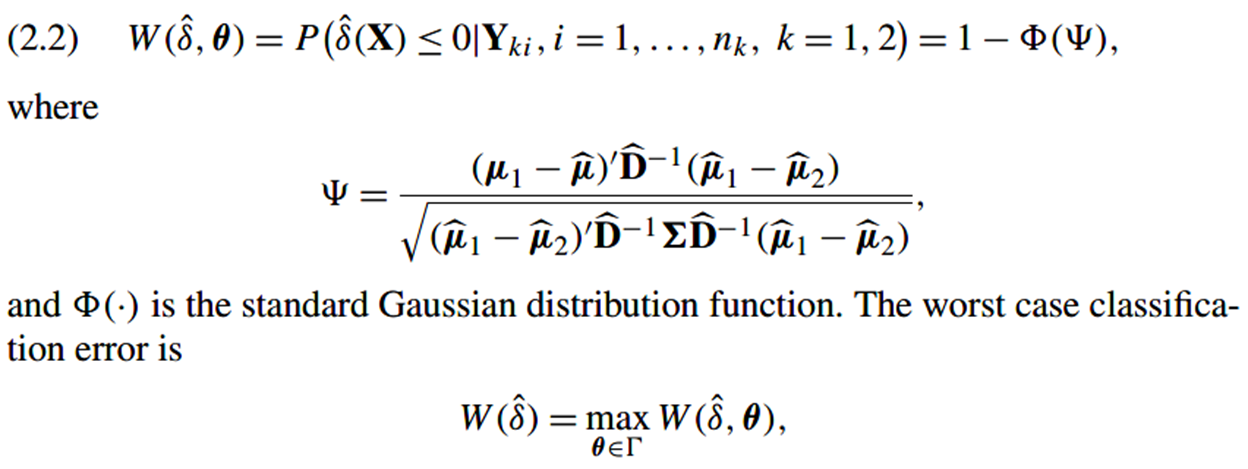
\includegraphics[width=0.9\linewidth]{image001.png}
		\end{figure}
	\end{frame}

	\begin{frame}
		\frametitle{Impact of High Dimensionality}
		Let $\bm{R} = \bm{D}^{-1/2}\bm{\Sigma}\bm{D}^{-1/2}$ be the correlation matrix, $\lambda_{max}(\bm{R})$ be its largest eigenvalue, and $\bm{\alpha} = \bm{\mu}_1 - \bm{\mu}_2$. Consider the parameter space:
		\begin{figure}
			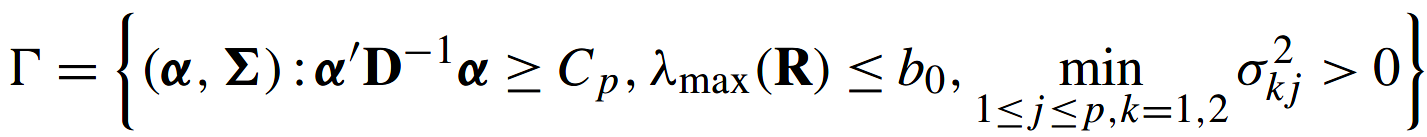
\includegraphics[width=0.8\linewidth]{image002.png}
		\end{figure}
		\begin{itemize}
			\item
			First term: imposes a lower bound on the strength of signals
			\item
			Second term: requires the maximum eigenvalue of $\bm{R}$ is upper bounded. (But there's no lower bound, the condition number can still diverge)\item
			Third term: ensures that there are no deterministic features that make classification trivial and $\bm{D}$is always invertible. 	
		\end{itemize}
		Then consider the asymptotic behavior of $W(\hat{\delta}, \bm{\theta})$ and $W(\hat{\delta})$.
	\end{frame}

	\begin{frame}
		\frametitle{Impact of High Dimensionality}
		\begin{figure}
			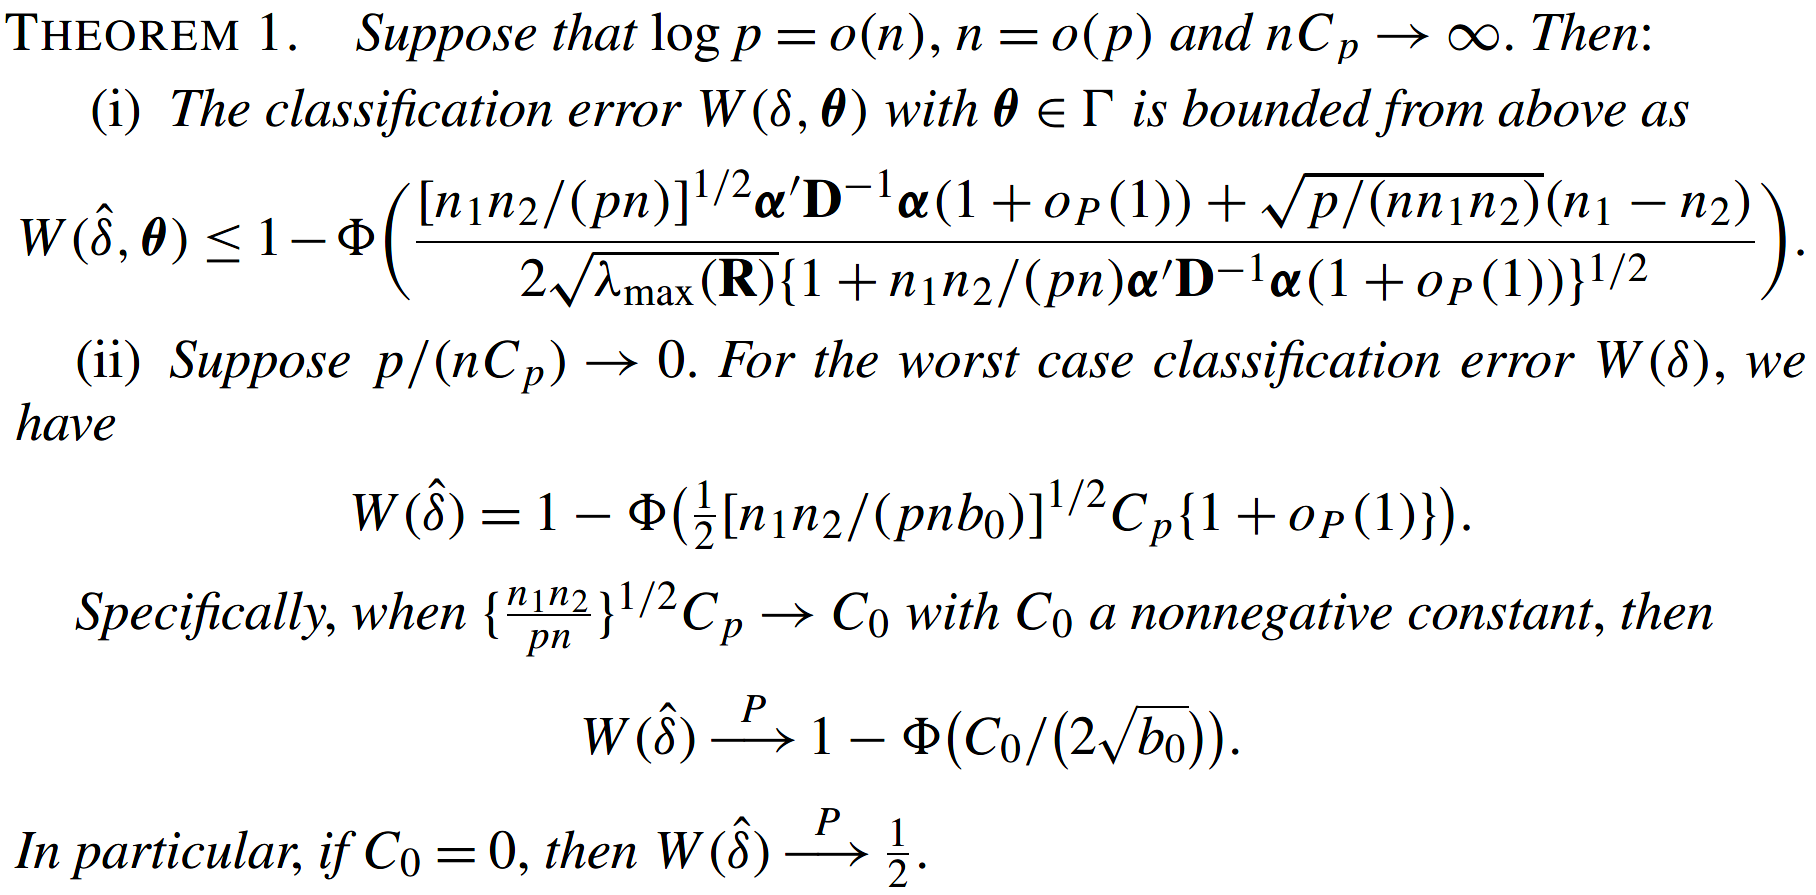
\includegraphics[width=0.9\linewidth]{image003.png}
		\end{figure}
	The independence rule $\hat{\delta}$ would be no better than the random guessing due to noise accumulation, unless the signal levels are extremely high.
	\end{frame}

	\begin{frame}
		\frametitle{Impact of High Dimensionality}
		Indeed, the discrimination based on linear projections to almost all directions performs nearly the same as random guessing (caused by noise accumulation in the estimation of $\bm{\mu}_1$ and $\bm{\mu}_2$)
		\begin{figure}
			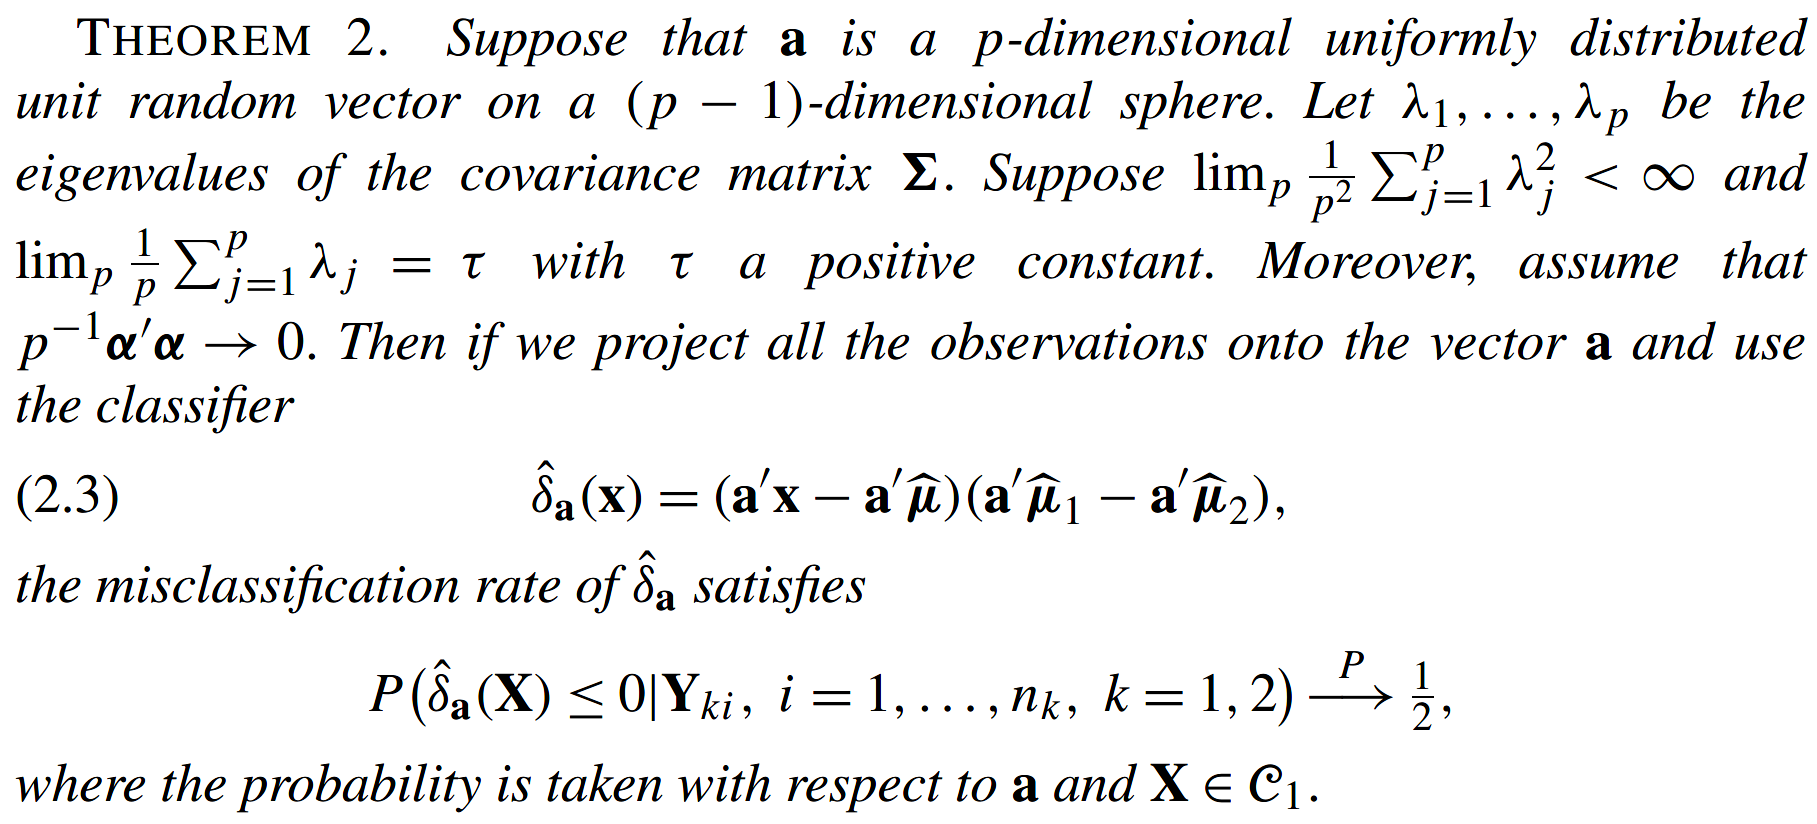
\includegraphics[width=0.9\linewidth]{image004.png}
		\end{figure}
	\end{frame}
	
	\section{Feature Selection by two-sample t-test}
	\begin{frame}
		\frametitle{Feature Selection by two-sample t-test}
		The 2 sample t-statistic for feature $j$ is defined as
		$$T_j = \frac{\bar{Y}_{1j} - \bar{Y}_{2j}}{\sqrt{S^2_{1j}/n_1 + S^2_{2j}/n_2}}$$  
		Relax the normality assumption: just assume the noise vector $\bm{\epsilon}_{ki}$ are $i.i.d.$ within class with mean $\bm{0}$ and covariance $\bm{\Sigma}_k$, and are independent between classes. Consider the following condition:
		\begin{figure}
			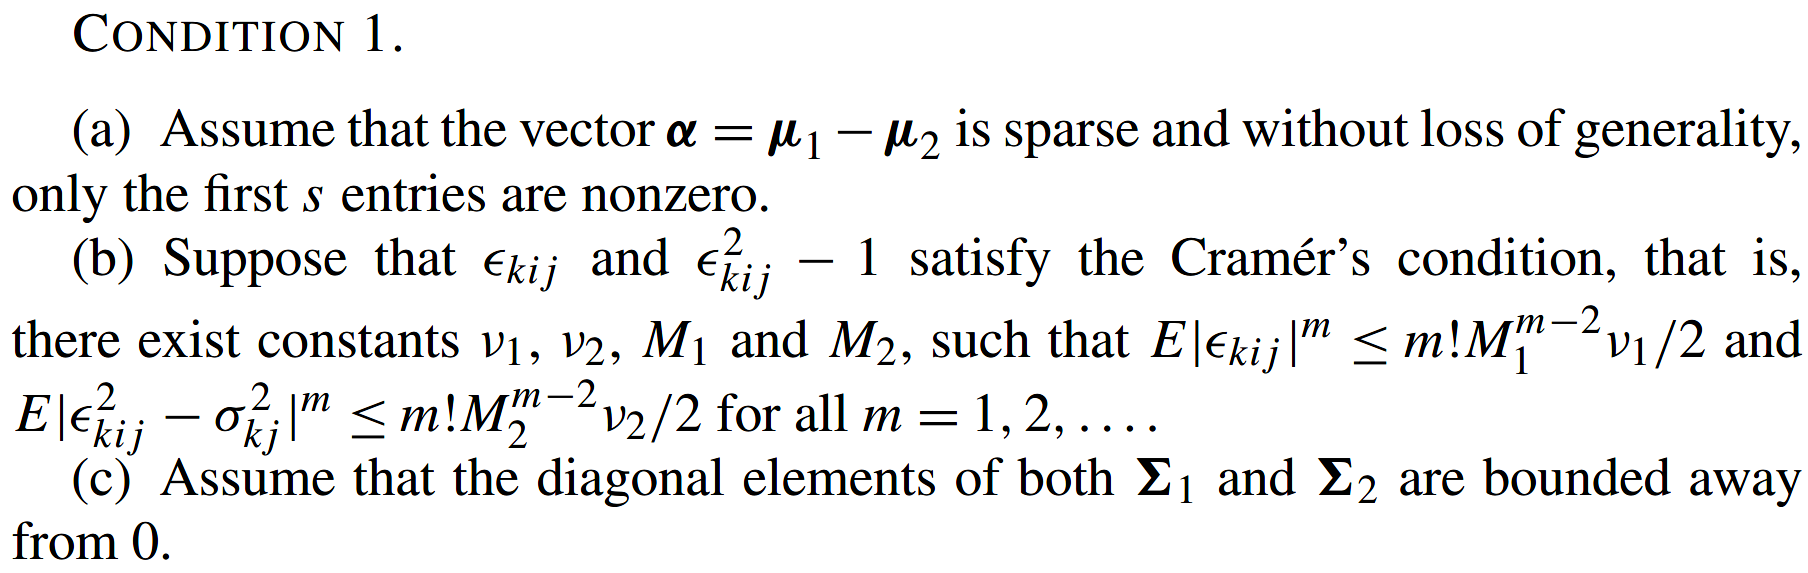
\includegraphics[width=0.9\linewidth]{image005.png}
		\end{figure}
	\end{frame}
	
	
	\begin{frame}
		\frametitle{Feature Selection by two-sample t-test}
		Under the condition on the previous slide, we  can show that the t-test can pick up all important features $w.p.1.$ ($c_1\leq n_1/n_2\leq c_2$ and $n = n_1 + n_2$)
		\begin{figure}
			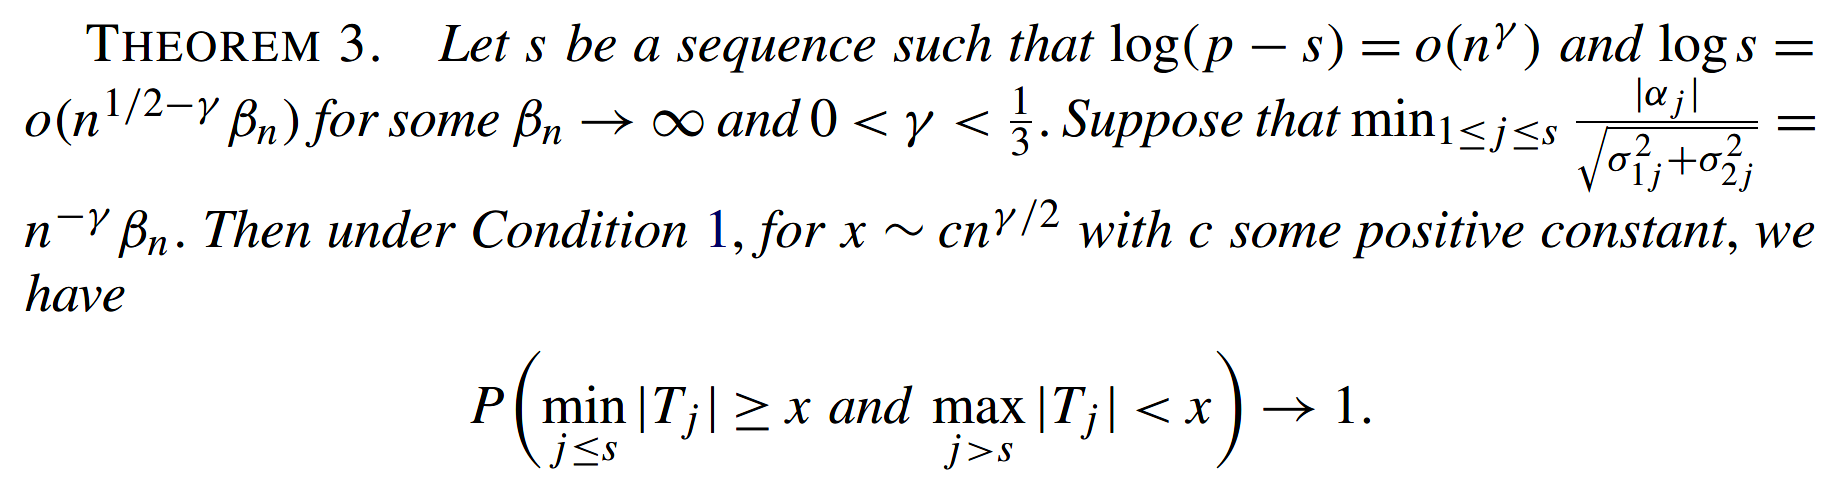
\includegraphics[width=1\linewidth]{image006.png}
		\end{figure}
	\end{frame}
	
	\section{Features Annealed Independence Rules}
	\begin{frame}
		\frametitle{Features Annealed Independence Rules}
		Just apply the independence classifier to the selected features $\rightarrow$ Featured Annealed Independence Rule (FAIR).\\
		\vspace{\baselineskip}
		In many application, $\bm{\alpha} = \bm{\mu}_1 - \bm{\mu}_2$ are sparse $\rightarrow$ the noise accumulation can exceed the signal accumulation for faint features $\rightarrow$ further single out the most important features to reduce misclassification rate, after using t-test.\\
		\vspace{\baselineskip}
		If $\bm{\Sigma}_1 = \bm{\Sigma}_2 = \bm{I}$, and is known, the independence classifier $\hat{\delta}$ becomes the nearest centroids classifier
		$$\hat{\delta}_{NC}(\bm{x}) = (\bm{x} - \hat{\bm{\mu}})'(\hat{\bm{\mu}}_1 - \hat{\bm{\mu}}_2)$$
		If only the first $m$ dimensions are used in the classification, the corresponding features annealed independence classifier becomes
		$$\hat{\delta}^m_{NC}(\bm{x}) = (\bm{x}^m - \hat{\bm{\mu}}^m)'(\hat{\bm{\mu}}_1^m - \hat{\bm{\mu}}_2^m)$$
	\end{frame}
	
	
	\begin{frame}
		\frametitle{Features Annealed Independence Rules}
		The classification error for the truncated classifier is: 
		\begin{figure}
			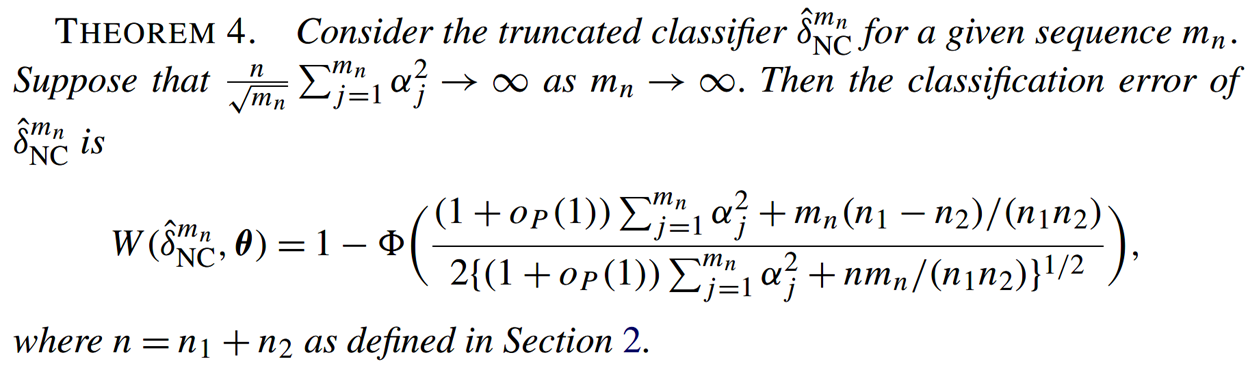
\includegraphics[width=1\linewidth]{image007.png}
		\end{figure}
		This theorem tells us that the ideal choice on the number of features is
		\begin{figure}
			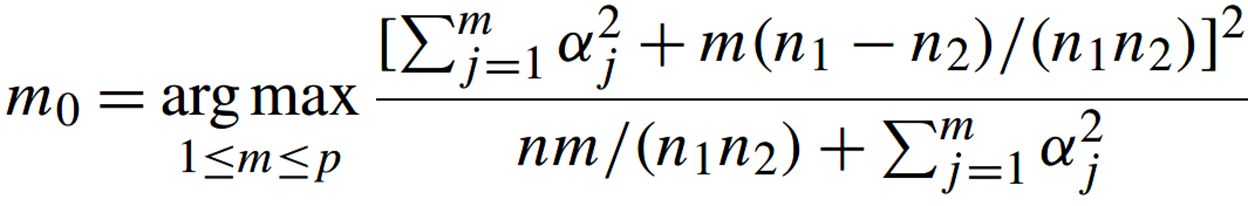
\includegraphics[width=.7\linewidth]{image008.png}
		\end{figure} 
	\end{frame}
	
	\begin{frame}
		\frametitle{Features Annealed Independence Rules}
		When $n_1 = n_2$, the expression reduces to $m_0 = \text{argmax}_{1\leq m\leq p}\frac{(m^{-1/2}\sum_{j=1}^{m}\alpha_j^2)^2}{2/n + \sum_{j=1}^{m}\alpha_j^2/m}$. The term $m^{-1/2}\sum_{j=1}^{m}\alpha_j^2$ reflects the trade-off between the signal and noise as dimensionality $m$ increases.\\
		\vspace{\baselineskip}
		An ideal classifier $\hat{\delta}_{NC}$ is to select a subset $A = \{j: |\alpha_j| > a\}$ and use this subset to construct independence classifier. The oracle classifier can be written as 
		\begin{figure}
			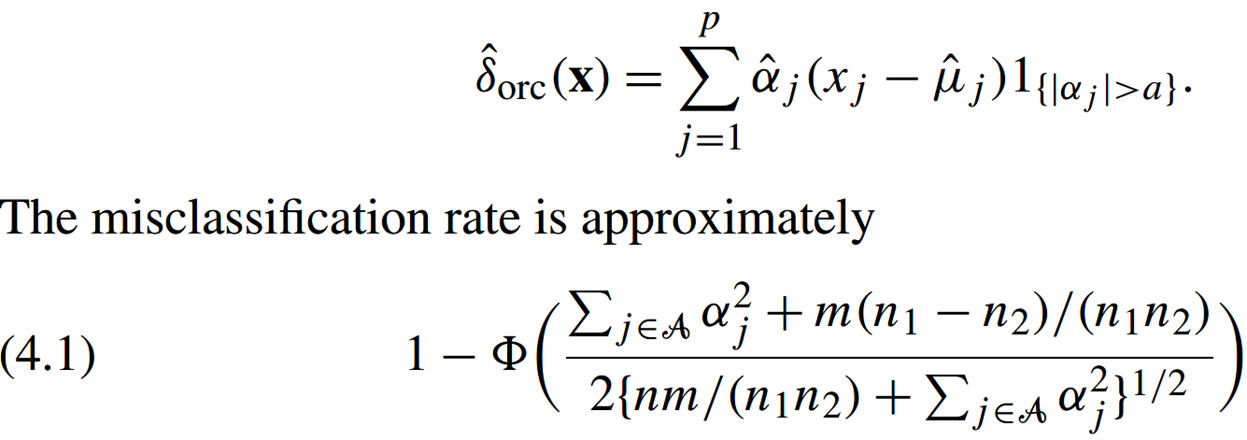
\includegraphics[width=.7\linewidth]{image009.png}
		\end{figure} 
		when $\frac{n}{\sqrt{m}}\sum_{j \in A}\alpha_j^2 \to \infty$ and $m \to \infty$.
	\end{frame}
	
	\begin{frame}
		\frametitle{Features Annealed Independence Rules}
		In practice, we have no such an oracle, and selecting the subset $A$ is difficult. Then just use the estimator-plug-in version: FAIR based on the hard thresholding:
		\begin{figure}
			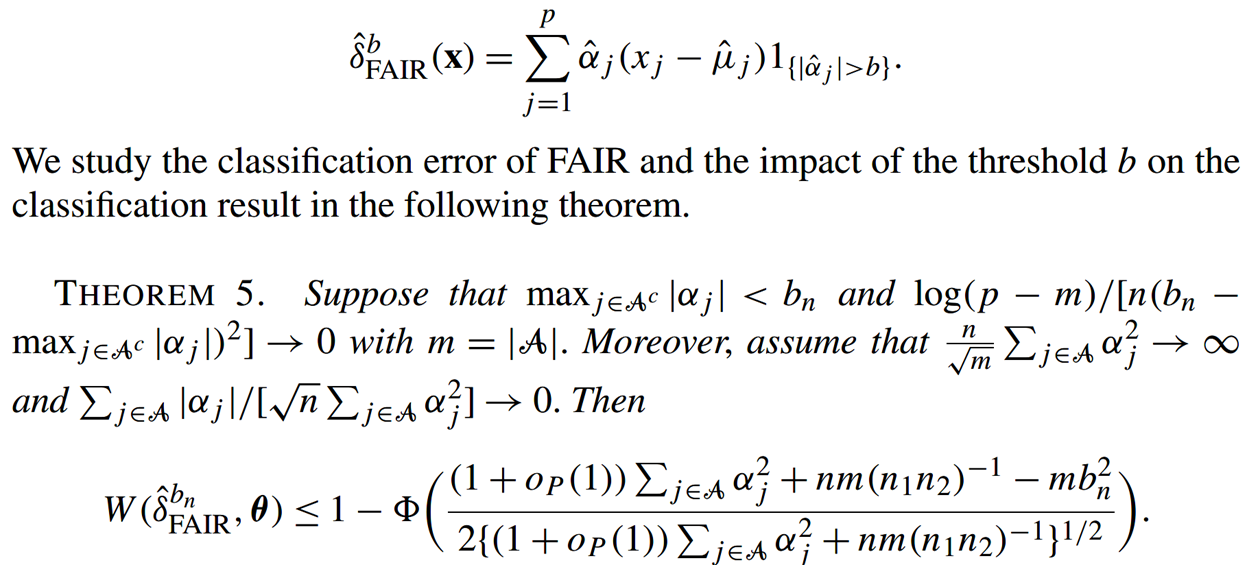
\includegraphics[width=.9\linewidth]{image010.png}
		\end{figure}
	\end{frame}
	
	\begin{frame}
		\frametitle{Features Annealed Independence Rules}
		Comment: The upper bound of $W(\hat{\delta}^{b_n}_{FAIR}, \bm{\theta})$ is greater than $W(\hat{\delta}^{m_n}_{NC}, \bm{\theta})$ (Theorem 4). This is expected as estimating the set $A$ increases the classification error.\\
		\vspace{\baselineskip}
		When the common covariance matrix is different from identity, FAIR takes a slightly different form:
		\begin{figure}
			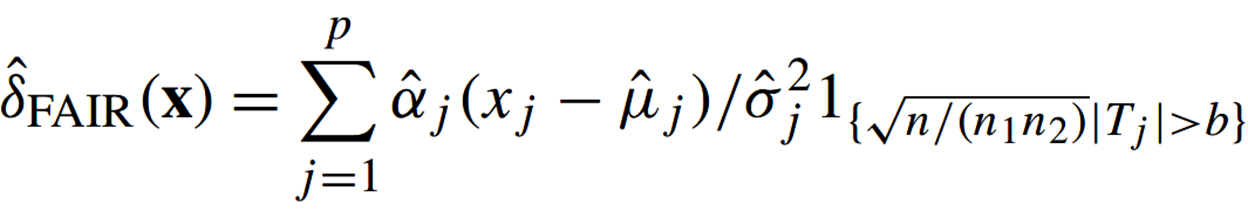
\includegraphics[width=.7\linewidth]{image011.png}
		\end{figure}
		, where $T_j$ is the two-sample t-statistic. 
	\end{frame}
	
	\begin{frame}
		\frametitle{Features Annealed Independence Rules}
		The number of features can be selected by minimizing the upper bound of the classification error. The optimal $m$ is:
		\begin{figure}
			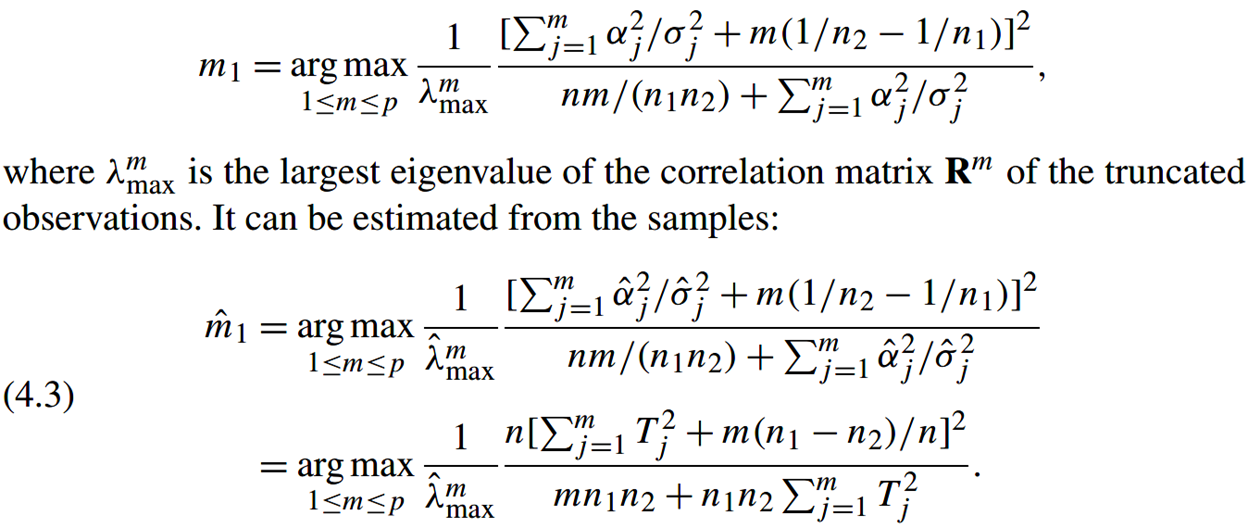
\includegraphics[width=.9\linewidth]{image012.png}
		\end{figure}
	\end{frame}
	
	\section{Numerical Studies}
	\begin{frame}
		\frametitle{Simulation}
		The big picture of the simulation:
		\begin{itemize}
			\item 
			The mean vector $\bm{\mu}_1$ is $(1-c)\delta_0 + \frac{c}{2}\exp(-2|x|)$, while $\bm{\mu}_2 = \bm{0}$.
			\item
			$n_1 = 30$ and $n_2 = 30$ for training. Seperate 200 samples are generated from each class as test dataset.
			\item
			Set $p = 4500$ and $c = 0.02$: around 90 signal features on an average, many of which are weak signals.
		\end{itemize}
	\begin{figure}
		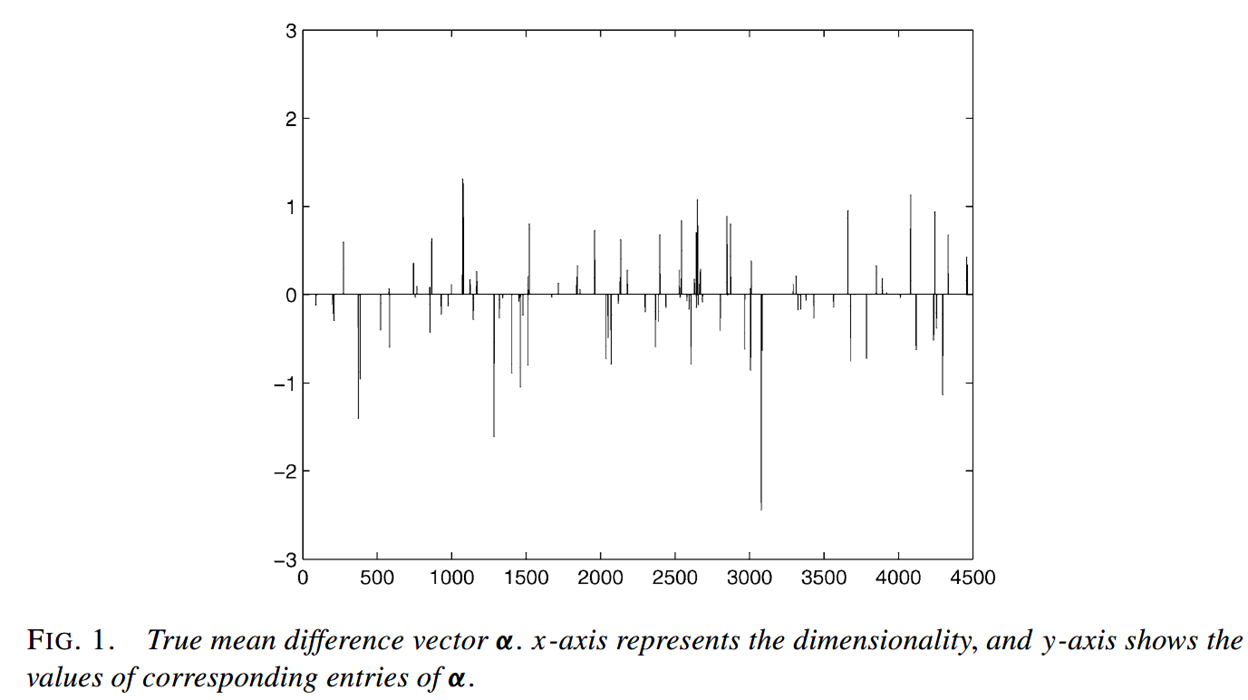
\includegraphics[width=.7\linewidth]{image013.png}
	\end{figure}
	\end{frame}
	
	\begin{frame}
		\frametitle{Simulation}
		Number of features vs. misclassification rates (averages + 2 standard errors) over 100 simulations.
		\begin{itemize}
			\item
			row 1: ordered by t-statistic (equivalently, $\hat{\bm{\alpha}}$, estimated mean differernces) 
			\item
			row 2: ordered by true $\bm{\alpha}$ 
		\end{itemize}
		\begin{figure}
			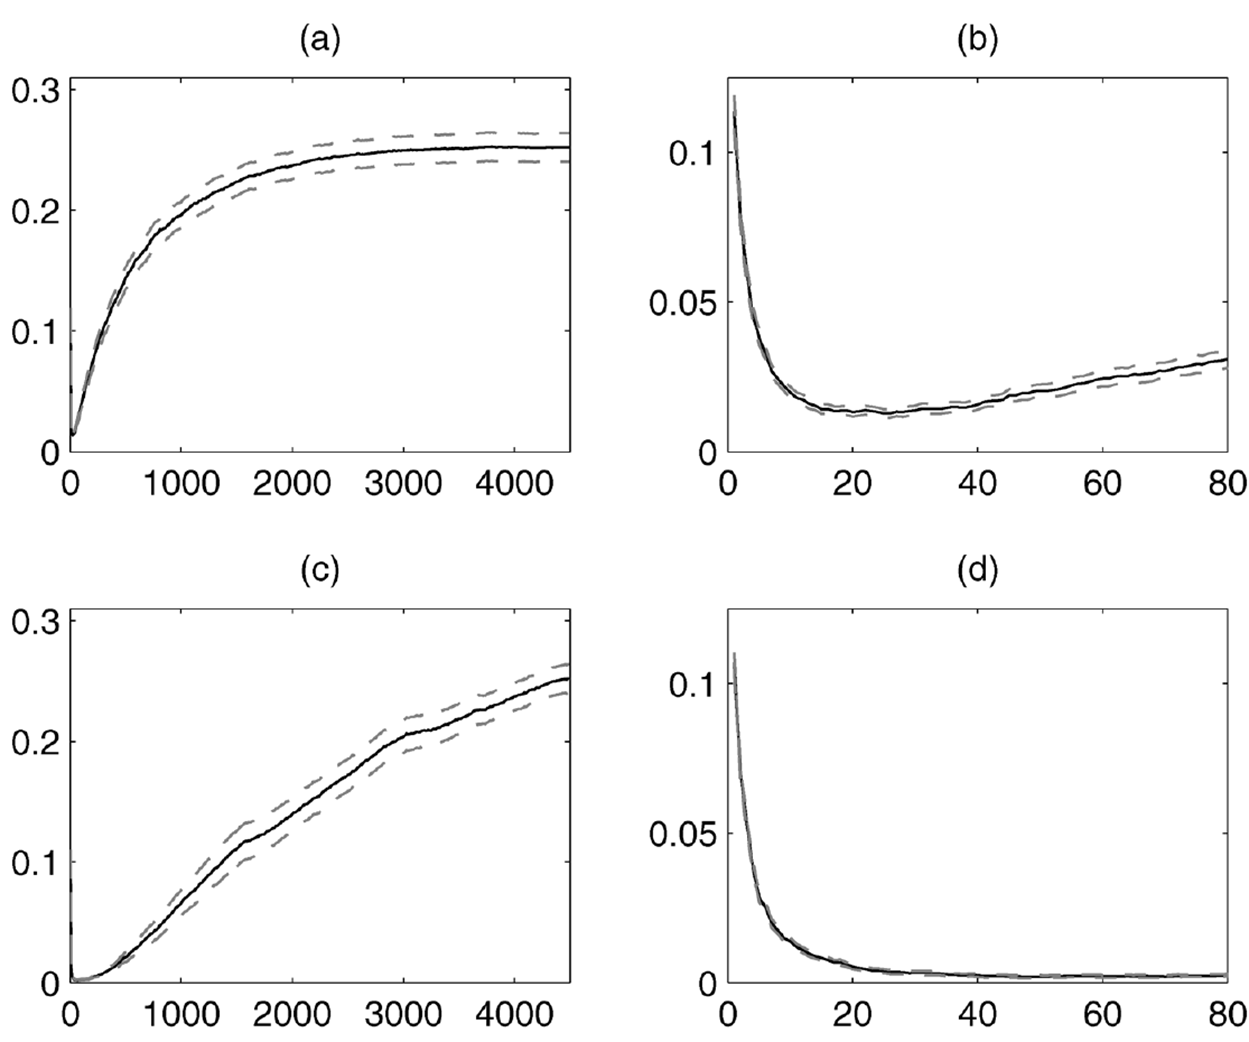
\includegraphics[width=.5\linewidth]{image014.png}
		\end{figure}
	\end{frame}
	
	\begin{frame}
		\frametitle{Simulation}
		Comments:
		\begin{itemize}
			\item
			Classification results of FAIR are close to those of the oracle -assisted independence classifier.
			\item
			m increase increases $\rightarrow$ misclassification rate increases 
			\item
			min = 0.0128 in upper, min = 0.0020 in lower.
			\item
			when all features are included ($m = 4500$),
			MR = 0.2522.
			\item
			When we decrease the signal levels/ increase the dimensionality, MR tend to 0.5.
			\item
			Similar results based on projected samples. 
		\end{itemize}
	\end{frame}
	
	\begin{frame}
		\frametitle{Simulation}
		What about the proposed method for selecting features in FAIR? Compare their method (thick) to nearest shrunken centroids method (NSC, thin). \textbf{Upper}: number of chosen features over 100 simulations; \textbf{Lower}: Classification error.
		\begin{figure}
			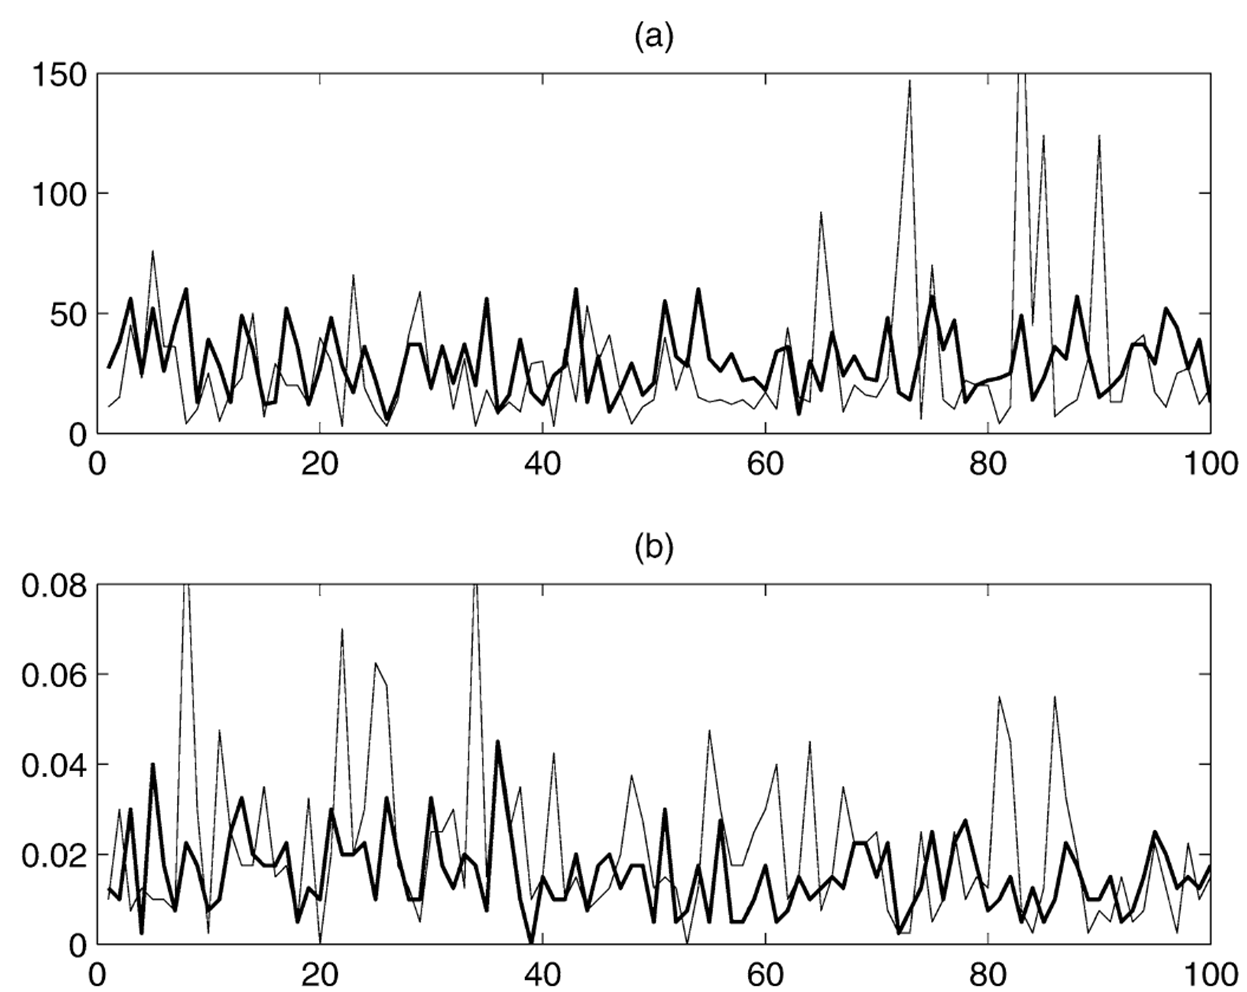
\includegraphics[width=.4\linewidth]{image015.png}
		\end{figure}
		FAIR: mean number of feature (29.71), mean MR (0.0154, sd = 0.0085)\\
		NSC: mean number of feature (28.43), mean MR (0.0216, sd = 0.0179)
	\end{frame}
	
	\begin{frame}
		\frametitle{Application 1: Leukemia data}
		7129 genes ($p$), 72 samples (47 in ALL and 25 in AML). 27 in ALL and 11 in AML are set to be training.
		\begin{figure}
			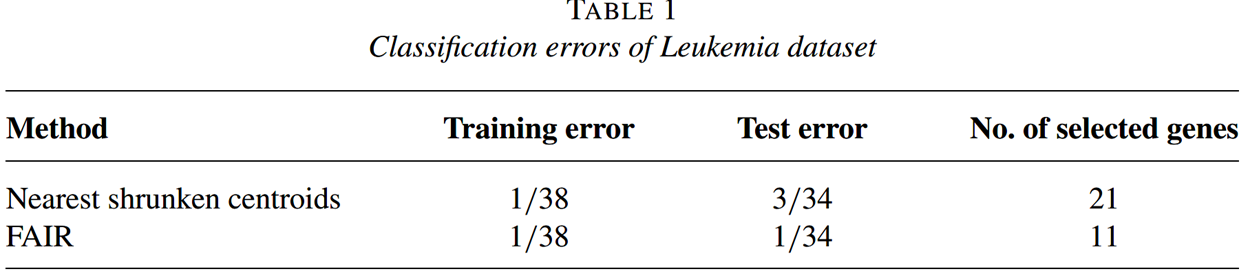
\includegraphics[width=.8\linewidth]{image016.png}
		\end{figure} 
	\end{frame}
	
	\begin{frame}
		\frametitle{Application 1: Leukemia data}
		Further set different proportion of training ($100\gamma\%$). idff = FARI - NSC; IR = independence rule (all features)
			\begin{figure}
			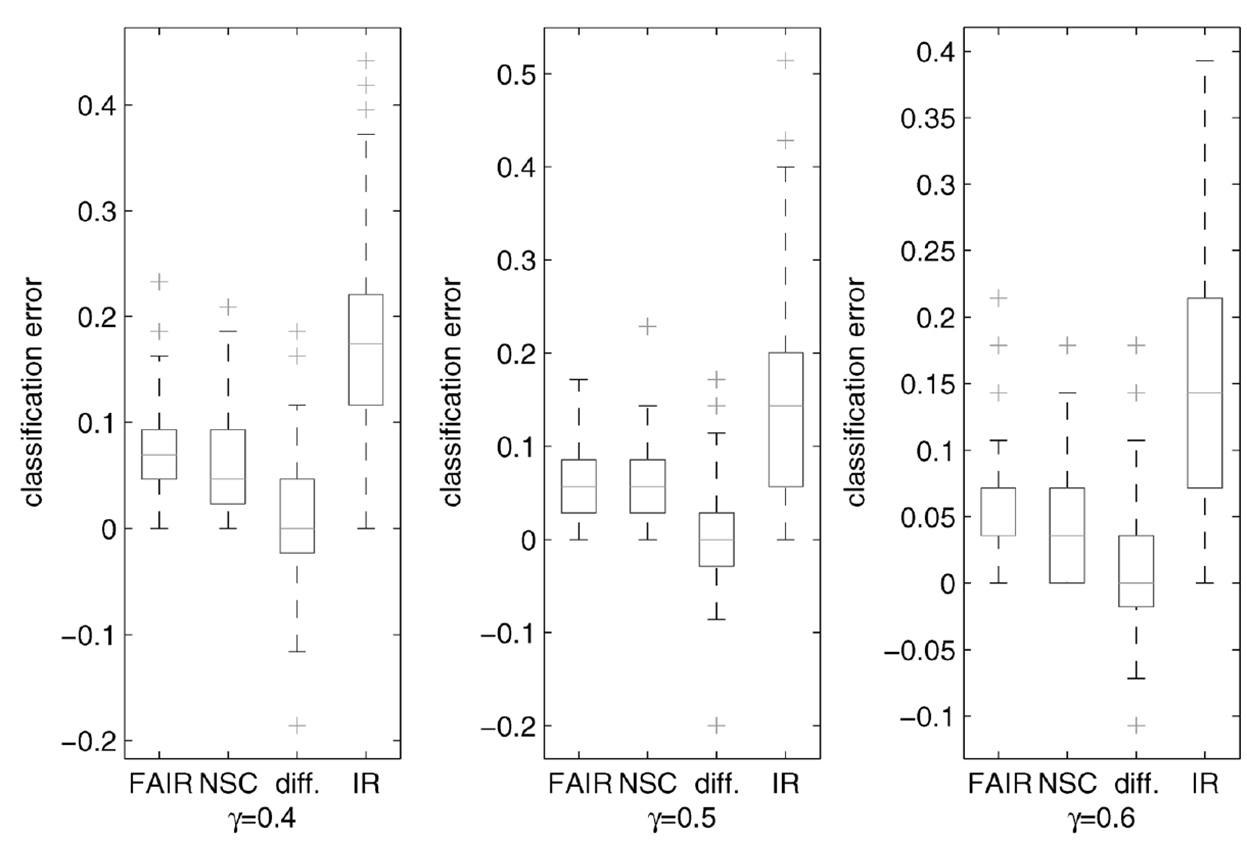
\includegraphics[width=.8\linewidth]{image017.png}
			\end{figure} 
	\end{frame}
	
	\begin{frame}
		\frametitle{Application 1: Leukemia data}
		\begin{figure}
			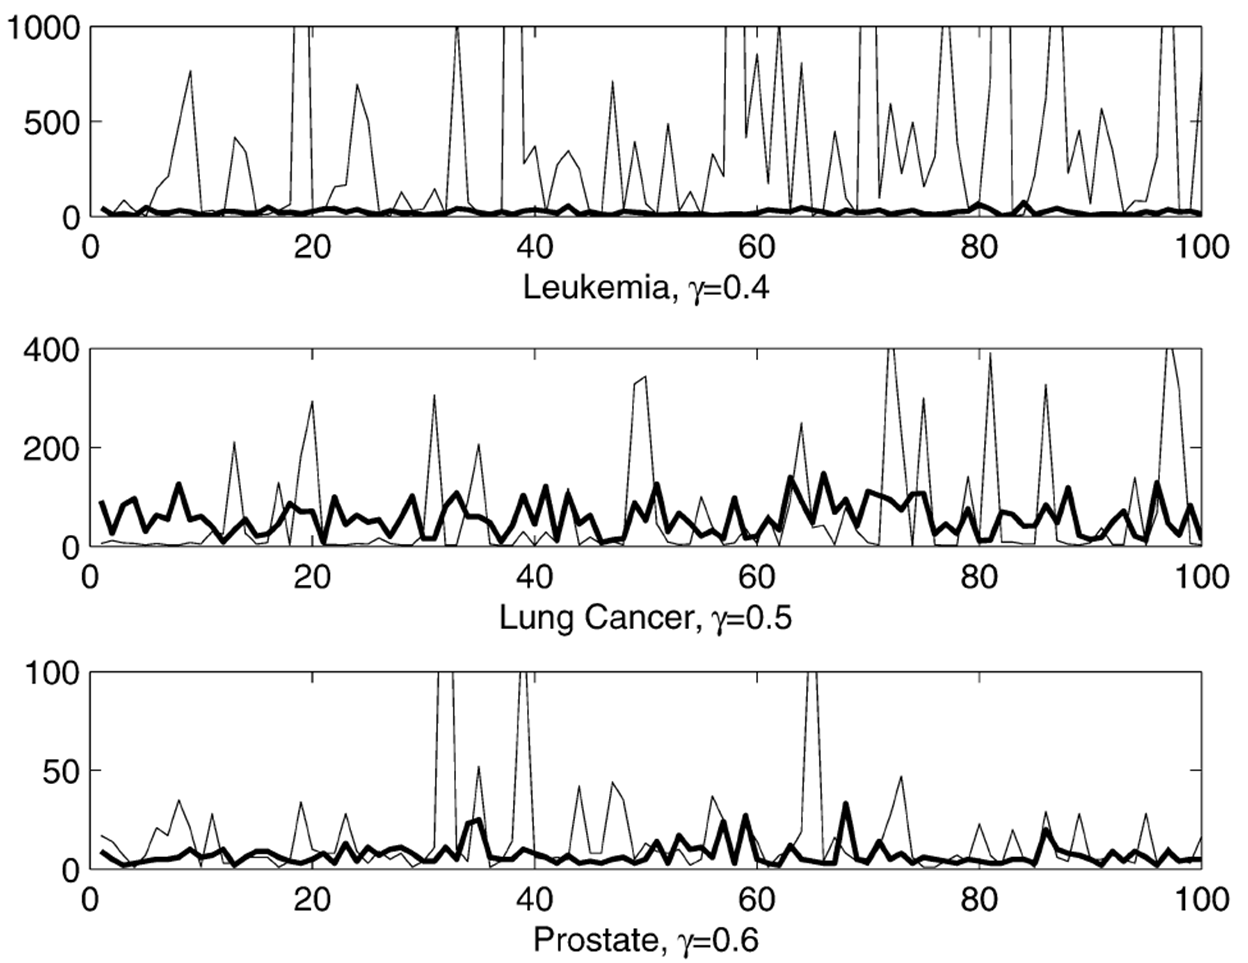
\includegraphics[width=.7\linewidth]{image018.png}
		\end{figure} 
		number of features: NSC is not good at feature selection.
	\end{frame}
	
	
	\begin{frame}
		\frametitle{Application 2: Lung Cancer data}
	\begin{figure}
		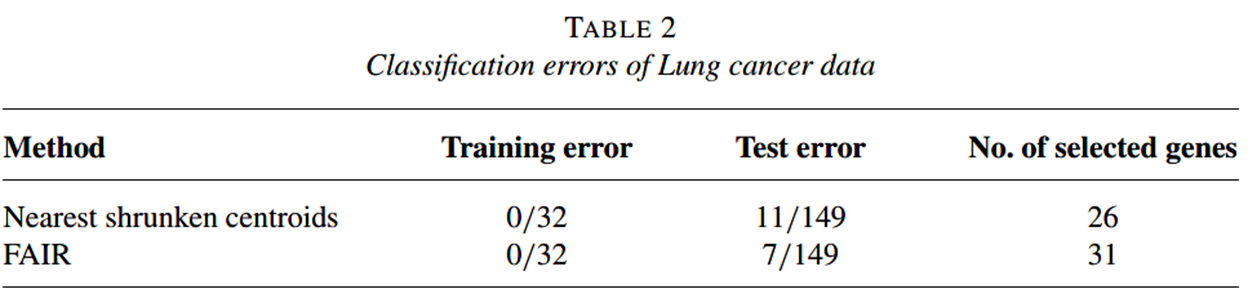
\includegraphics[width=.8\linewidth]{image019.png}
		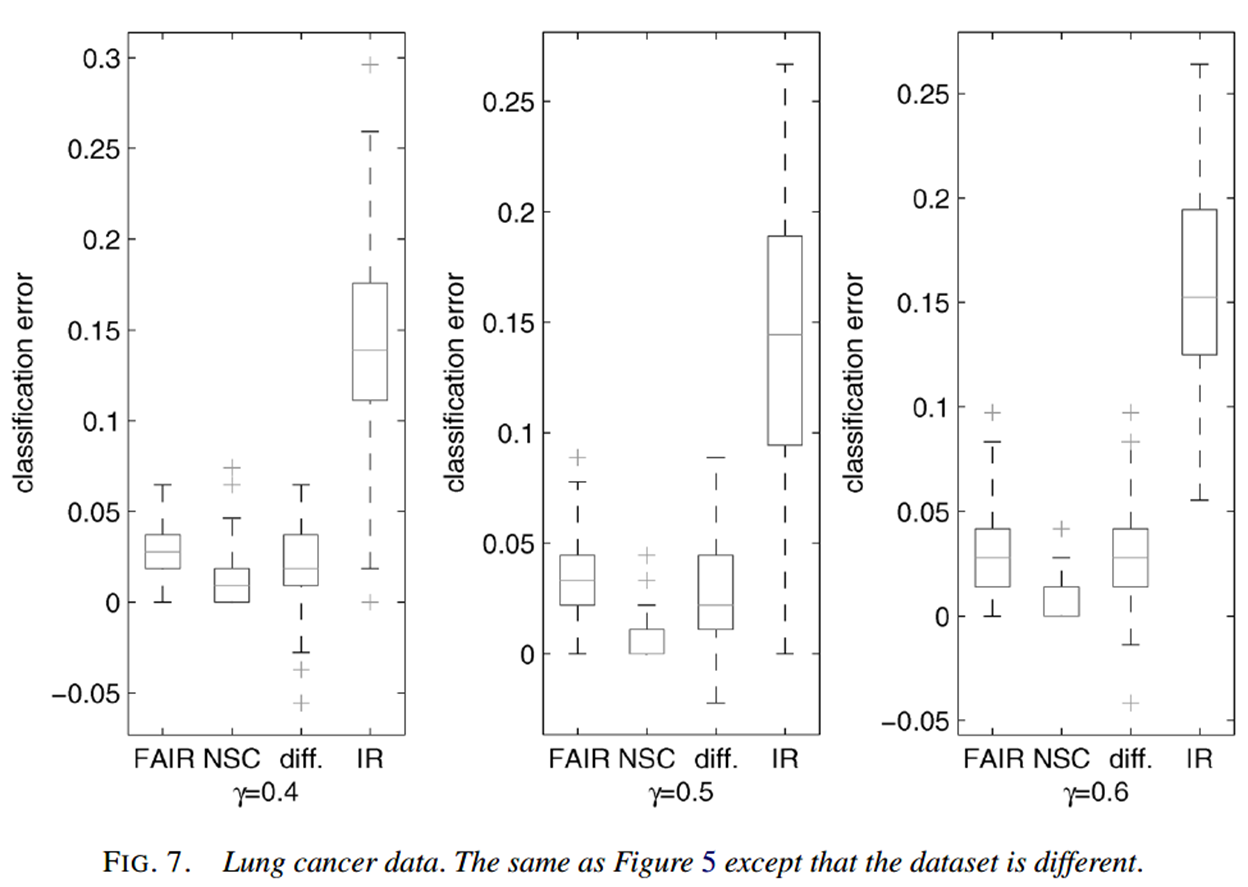
\includegraphics[width=.7\linewidth]{image020.png}
	\end{figure} 	
	\end{frame}
	
	\begin{frame}
		\frametitle{Application 3: Prostate Cancer data}
	\begin{figure}
		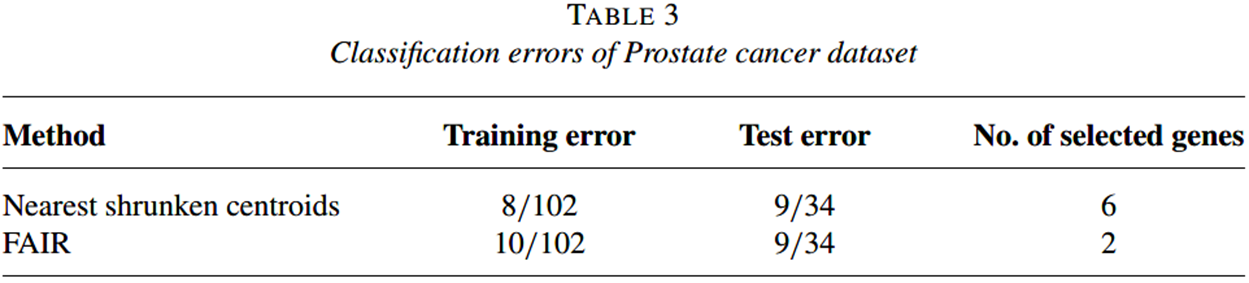
\includegraphics[width=.8\linewidth]{image021.png}
		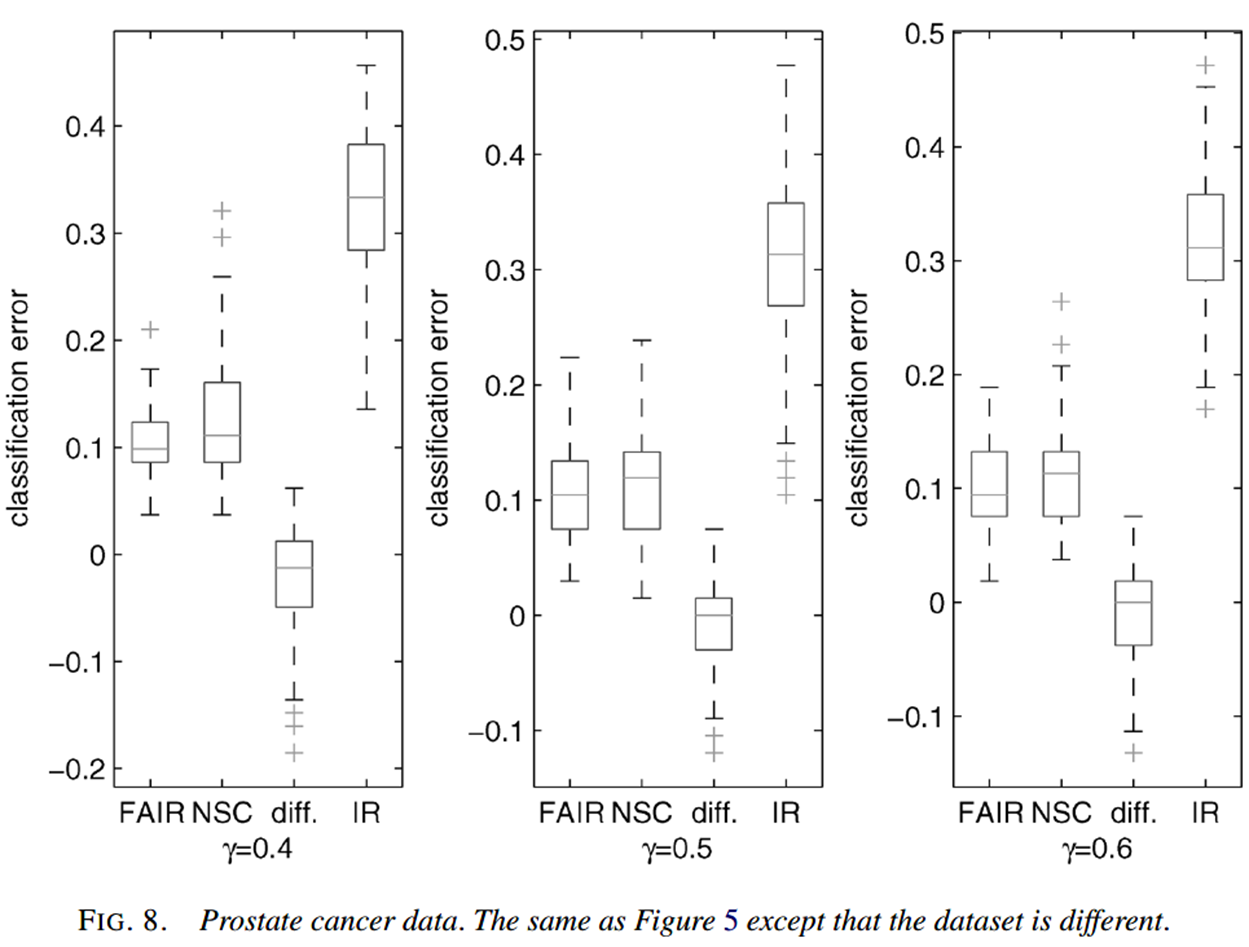
\includegraphics[width=.7\linewidth]{image022.png}
	\end{figure} 	
	\end{frame}
	
	
\end{document}